% -*- coding: utf-8 -*-
\documentclass{article}
\usepackage{polski}
%\usepackage[T1]{fontenc}
%\usepackage[utf8]{inputenc}
\usepackage{xltxtra}
\usepackage{listings}
\usepackage{fullpage}
\usepackage{graphicx}
\usepackage{color}
\usepackage{amsmath}
\usepackage{amsthm}
\usepackage{indentfirst}
\usepackage{hyperref}
\newtheorem{twi}{Twierdzenie}
\author{Karol Piotrowski, Krzysztof Pater}
\title{Algorytmy i Struktury Danych, projekt\\ Algorytm Dinica znajdowania największego przepływu}
\begin{document}
\maketitle
\section{Wstęp}
Niedługo minie 60 lat, od kiedy Ford i Fulkerson dowiedli w pracy [1] twierdzenia:
\begin{twi} Niech $S=(G,c)$ będzie siecią przepływową. Wówczas jeśli $A, V\setminus A$ jest przekrojem minimalnym ze względu na wartość $c(A)=\sum_{u \in A. v\notin A} c(u,v)$ to dla dowolnego przepływu $f$ w sieci $S$ zachodzi nierówność $c(A) \leq |f|$, a ponadto istnieje przepływ maksymalny, dla którego zachodzi równość.
  \end{twi}
Nietrywialną częścią było wykazanie, że maksymalny przepływ rzeczywiście istnieje (minimalny przekrój nie trudno sobie wyobrazić biorąc pod uwagę fakt, że jest skończona liczba zbiorów wierzchołków), zaś zaproponowany przez Forda i Fulkersona algorytm miał złożoność czasową $O(|V|\cdot \max_{e\in E} c(E))$, zatem poza szczególnymi przypadkami niewielkie zastosowanie praktyczne. Od tego czasu powstało wiele algorytmów zarówno teoretycznych jak i praktycznych, a w 2013 roku świat obiegła informacja o prawie liniowym aproksymacyjnym algorytmie znajdowania maksymalnego przepływu (patrz praca [2]). Celem tego projektu będzie zbadanie empiryczne jednego z podstawowych algorytmów, opracowanego przez Dinica. Będziemy zajmować się wersją klasyczną, działającą w czasie $O(|V|^2|E|)$, gdyż wersja ta jest prostsza i bardziej czytelna w implementacji niż np. modyfikacja znana jako algorytm trzech Hindusów (MKM, patrz [3]), która działa w czasie $O(|V|^3)$, a więc powinna sprawdzać się lepiej dla sieci wypełnionych krawędziami (takich, że $|E| = \Omega(|V|^2)$). 

\section{Opis i analiza algorytmu}
  Omówimy krótko klasyczną wersję algorytmu Dinica dla sieci nieskierowanych. Implementacji dokonano ze względów dydaktycznych w języku Python, z zastosowaniem wbudowanych dynamicznych struktur danych (\texttt{list()} jako tablica, gdyż zgodnie ze standardem języka jest ona realizowana jako tablica dynamiczna z kosztem amortyzowanym zarówno zapisywania, jak i odczytywania $O(1)$ oraz \texttt{collections.deque} jako stos/kolejka, gdyż jest to w rzeczywistości lista dwukierunkowa). Do zapisu tablicy list sąsiedztwa w grafie użyto \texttt{list()} dla prostoty zapisu (i tak iterujemy prawie zawsze od początku listy i dopisujemy na ,,właściwym" końcu). 
  
Algorytm Dinica jest jednym z algorytmów wykorzystujących tzw. przepływy blokujące. \emph{Przepływ blokujący} to taki, w którym każda ścieżka od źródła do ujścia zawiera krawędź nasyconą (taką, że $f(u,v) = c(u,v)$).

Idea jest następująca: w każdej fazie działania algorytmu Dinica przeszukujemy sieć BFSem, przypisując wierzchołkom \emph{odległości od źródła}, przy czym odwiedzamy tylko wierzchołki, od których wychodzi krawędź nienasycona (taka, na której przepływ jest mniejszy od pojemności). Jeśli nie uda się znaleźć żadnej nienasyconej ścieżki od źródła do ujścia, to
oznacza, że przepływ jest maksymalny i algorytm kończy pracę. W innym wypadku bierzemy maksymalną możliwą wartość przepływu ze źródła i i próbujemy przepuścić ją przez ścieżkę blokującą. Realizowane jest to tym razem za pomocą rekurencyjnego przeszukiwania DFS. Istotne w działaniu algorytmu Dinica jest to, że w każdej fazie ścieżki blokujące są co raz dłuższe: dzięki temu algorytm zakończy się po skończonej liczbie kroków (można udowodnić, że dla grafu o $n$ wierzchołkach wystarczy $n-1$ kroków).

Poprawność działania  algorytmu jest jasna ze względu na fakt, że algorytm nie opuszcza pętli dopóki istnieje chociaż jedna ścieżka od źródła do ujścia na której istnieje krawędź nienasycona. Podstawowym faktem z teorii sieci przepływowych jest to, że przepływ jest maksymalny wtedy i tylko wtedy, gdy nie istnieje w nim ściezka rozszerzająca. Ponieważ ścieżka rozszerzająca jest blokująca, to brak ściezki blokującej oznacza brak ścieżki rozszerzającej. 

\section{Empiryczne testy stworzonej implementacji}
W wykonanej aplikacji ,,Algorytm Dinica" umieszczono możliwość wykonywania testów czasu działania algorytmu i generowania na ich podstawie wykresów. Ze względu na dużą złożoność obliczeniową i wymagania pamięciowe (ze względu na przechowywanie tablicy przepustowości potrzeba $O(|V|^2)$ pamięci) testy przeprowadzono dla zakresu do około 100 wierzchołków grafu. W pierwszej kolejności zbadano średni czas wykonania algorytmu dla $|V|=30$ i zmieniającej się liczby krawędzi:
\begin{center}
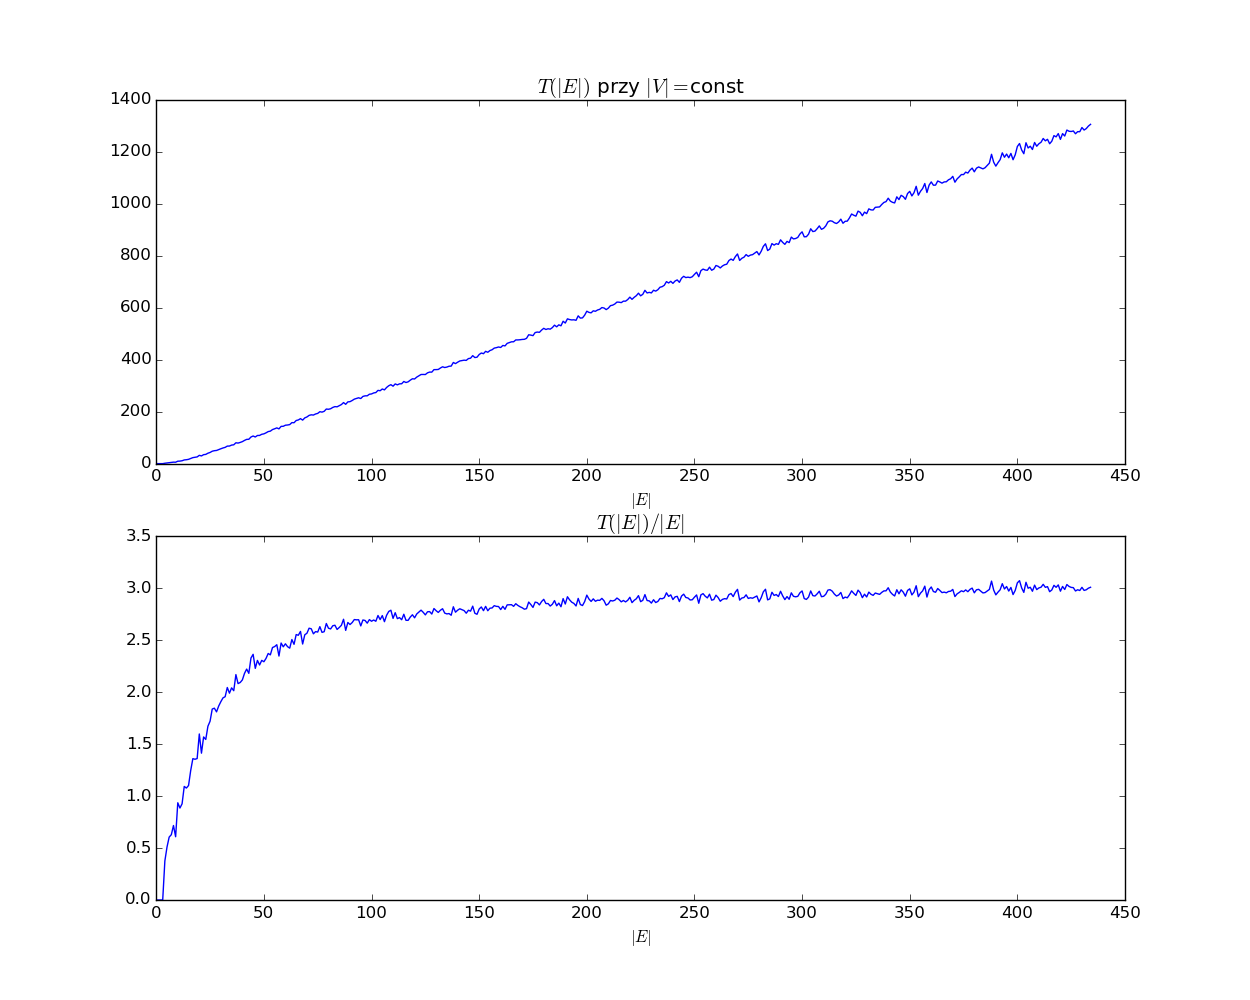
\includegraphics[scale=0.5]{constv.png}
\end{center}
Czas wykonania przedstawiono w jednostkach umownych--$T(|E|) = t(|E|)/t(3)$, gdzie $t$ jest średnim czasem pracy algorytmu w sekundach. Przedstawione dane doświadczalne ilustrują fakt, że przy ustalonym $|V|$ czas działania algorytmu jest liniowy ze względu na $|E|$ ($T(|E|)/|E|$ jest praktycznie stałe dla dużych $|E|$).

W następnej kolejności zbadano (i wyrażono w jednostkach umownych podobnie jak w poprzednim przypadku) czas działania algorytmu dla sieci o małej liczbie krawędzi ($|E| = O(|V|)$) dla $|V|\leq 100$, dane umieszczono na wykresie: 
\begin{center}


\begin{center}
\includegraphics[scale=0.5]{
\includegraphics[scale=0.5]{malee.png}
\end{center}
Jak widać, $T(|V|)/|V|^2$ jest stałe dla szerokiego zakresu $|V|$, co ilustruje kwadratową \emph{średnią} złożoność algorytmu dla $|E|=O(|V|)$. Oszacowanie pesymistyczne to $O(|V|^3)$, jednak przy losowym generowaniu sieci bardzo często algorytm zatrzymuje się szybciej, gdyż w ogóle nie ma drogi od źródła do ujścia. 

Jako ostatnie zbadano sieci bogate w krawędzi:
\begin{center}
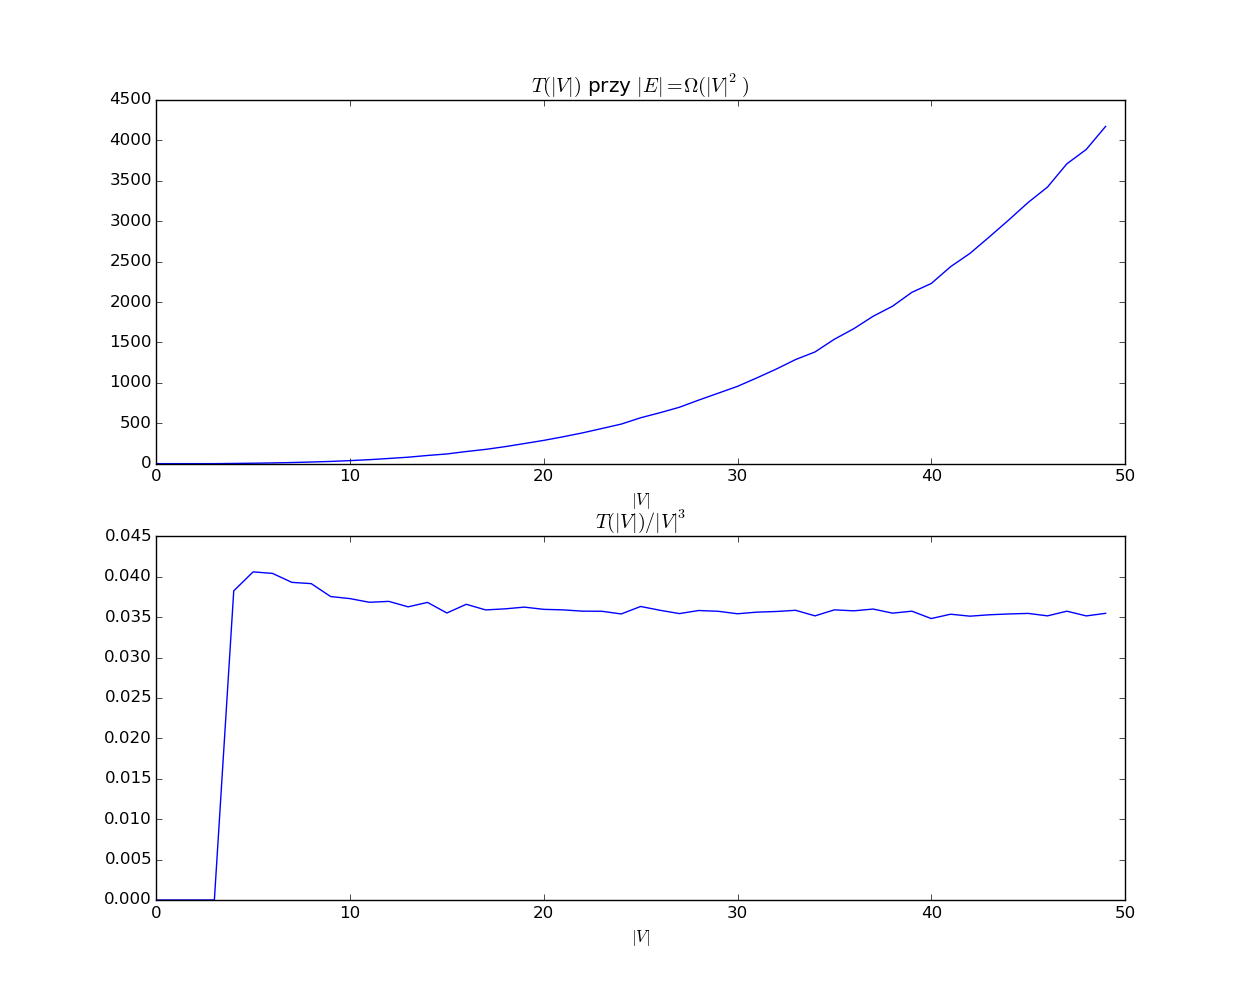
\includegraphics[scale=0.5]{duzee.png}
\end{center}
Dla bogatych w krawędzie sieci ($|E| = \Omega(|V|^2)$) otrzymano zachowanie się $T(|V|)$ jak $|V|^3$--obecna implementacja zdecydowanie gorzej radzi sobie z takimi sieciami. Podobnie, jak przy testach dla małej ilości krawędzi, otrzymaliśmy ze względu na fakt, że jest to złożononść średnia z losowo dobieranymi grafami i pojemnościami, złożoność lepsza od teoretycznej $O(|V|^4)$. 

\section{Wnioski}
Algorytm Dinica realizuje zadanie znajdowania największego przepływu w czasie wielomianowym, zależnym liniowo od liczby krawędzi. 
\end{document}
